\section{Mesh-based methods}

\begin{frame}{\appendixname~\theappendixframenumber~: Encoding - FEMs}\labelappendixframe{frame:encoding_fems}
	We want to project $f$ onto the vector subspace $V_N$ so that $f_\theta = p_{V_N}(f)$ \\	
	then $\forall i \in \{1,\dots,N\}$, we have
	\begin{align*}
		&\quad \langle f_\theta - f, \varphi_i \rangle = 0 \\
		\iff &\quad \langle f_\theta, \varphi_i \rangle = \langle f, \varphi_i \rangle \quad  \\
		\iff &\quad \sum_{j=1}^N(\theta_f)_j \langle \varphi_j, \varphi_i\rangle = \langle f, \varphi_i \rangle \\ 
		\iff &\quad M \theta_f = b(f) \\
		\iff &\quad \theta_f = M^{-1} b(f)
	\end{align*}	
	with 
	\begin{align*}
		M_{ij} &= \langle \varphi_i, \varphi_j\rangle = \int_{\Omega} \varphi_i(x) \varphi_j(x) \, dx \\
		b_i(f) &= \langle f, \varphi_i \rangle = \int_{\Omega} f(x) \varphi_i(x) \, dx
	\end{align*}	
\end{frame}
\addtocounter{appendixframenumber}{1}

\begin{frame}[allowframebreaks]{\appendixname~\theappendixframenumber~: Energetic form} \labelappendixframe{frame:minpb_galerkin}
	Let's compute the gradient of $J$ with respect to $v$ with
	\begin{equation*}
		J(v)=J_{in}(v)+J_{bc}(v)=\left(\frac{1}{2}\int_\Omega L(v)v - \int_\Omega fv\right) + \left(\frac{1}{2}\int_{\partial\Omega} R_{bc}(v)^2\right)
	\end{equation*}

	\begin{itemize}[\textbullet]
		\item First, let's calculate the differential of $J_{in}$ with respect to $v$.
		\begin{align*}
			J_{in}(v+\epsilon h)=\frac{1}{2} \int_{\Omega} (A\nabla(v+\epsilon h)) \cdot \nabla(v+\epsilon h) + c(v+\epsilon h)^2 - \int_{\Omega} f(v+\epsilon h)
		\end{align*}
		
		By bilinearity of the scalar product and by symmetry of $A$, we finally obtain
		\begin{equation*}
			\mathcal{D}J_{in}(v)\cdot h = \lim_{\epsilon\rightarrow 0}\frac{J_{in}(v+\epsilon h)-J_{in}(v)}{\epsilon} = \int_{\Omega} (-\nabla\cdot(A\nabla v) + cv - f)h
		\end{equation*}
		
		And thus
		\begin{equation*}
			\nabla_v \; J_{in}(v) = L(v) - f = R_{in}(v)
		\end{equation*}
	
		\newpage
		
		\item In the same way, we can compute the differential of $J_{bc}$ with respect to $v$.
		\begin{align*}
			J_{bc}(v+\epsilon h)=\frac{1}{2} \int_{\partial\Omega} v^2+2\epsilon vh +\epsilon^2 h^2 - 2vg - 2\epsilon hg+g^2
		\end{align*}
		
		Then
		\begin{align*}
			\mathcal{D}J_{bc}(v)\cdot h =  \lim_{\epsilon\rightarrow 0}\frac{J_{bc}(v+\epsilon h)-J_{bc}(v)}{\epsilon} = \int_{\partial\Omega} (v-g)h
		\end{align*}
		
		And thus
		\begin{align*}
			\nabla_v \; J_{bc}(v) = (v-g) = R_{bc}(v) 
		\end{align*}
	\end{itemize}
	
	Finally
	\begin{equation*}
		\nabla_v \; J(v) = \nabla_v \; J_{i}(v) + \nabla_v \; J_{bc}(v) = R(v)
	\end{equation*}
\end{frame}
\addtocounter{appendixframenumber}{1}

\begin{frame}{\appendixname~\theappendixframenumber~: Galerkin Projection}\labelappendixframe{frame:galerkin_proj}
	Let's compute the gradient of $J$ with respect to $\theta$ with
	\begin{equation*}
		J(\theta)=J_{in}(\theta)=\frac{1}{2}\int_\Omega L(u_\theta)v_\theta - \int_\Omega fv_\theta
	\end{equation*}
	First, we define
	\begin{equation*}
		v_\theta=\sum_{i=1}^{N} \theta_i \varphi_i=\theta\cdot\varphi \qquad \text{and} \qquad v_{\theta+\epsilon h}=(\theta+\epsilon h)\cdot\varphi=v_\theta+\epsilon v_h
	\end{equation*}
	Then since $A$ is symmetric
	\begin{equation*}
		\mathcal{D}J(\theta)\cdot h =\int_\Omega R(v_\theta)v_h =\sum_{i=1}^N h_i\int_\Omega R(v_\theta)\varphi_i
	\end{equation*}
	Finally
	\begin{align*}
		\nabla_\theta \; J(\theta) = \left(\int_\Omega R(v_\theta)\varphi_i\right)_{i=1,\dots,N}
	\end{align*}
\end{frame}
\addtocounter{appendixframenumber}{1}

\begin{frame}[allowframebreaks]{\appendixname~\theappendixframenumber~: Least-Square form}\labelappendixframe{frame:minpb_leastsquare}
	Let's compute the gradient of $J$ with respect to $v$ with
	\begin{equation*}
		J(v)=J_{in}(v)+J_{bc}(v)=\left(\frac{1}{2}\int_\Omega R_{in}(v)^2\right)+\left(\frac{1}{2}\int_{\partial\Omega} R_{bc}(v)^2\right)
	\end{equation*}
	\begin{itemize}[\textbullet]
		\item First, let's calculate the differential of $J_{in}$ with respect to $v$.
		\begin{align*}
			\mathcal{D}J_{in}(v)\cdot h &= \langle \nabla\cdot(A\nabla h), \nabla\cdot(A\nabla v) - cv +f \rangle+\langle ch, -\nabla\cdot(A\nabla v) + cv - f \rangle \\ 
			&= -\langle \nabla\cdot(A\nabla h), R_{in}(v) \rangle+\langle ch, R_{in}(v)\rangle \\ 
			&= \langle -\nabla\cdot(A\nabla R_{in}(v))+cR_{in}(v), h \rangle \\
			&= \langle L(R_{in}(v)), h \rangle
		\end{align*}
		And thus		
		\begin{equation*}
			\nabla_v \; J_{in}(v) = L(R_{in}(v))
		\end{equation*}
	
		\newpage
		
		\item In the same way, we can compute the differential of $J_{bc}$ with respect to $v$.
		\begin{align*}
			J_{bc}(v+\epsilon h)=\frac{1}{2} \int_{\partial\Omega} v^2+2\epsilon vh +\epsilon^2 h^2 - 2vg - 2\epsilon hg+g^2
		\end{align*}
		
		Then
		\begin{align*}
			\mathcal{D}J_{bc}(v)\cdot h =  \lim_{\epsilon\rightarrow 0}\frac{J_{bc}(v+\epsilon h)-J_{bc}(v)}{\epsilon} = \int_{\partial\Omega} (v-g)h
		\end{align*}
		
		And thus
		\begin{align*}
			\nabla_v \; J_{bc}(v) = (v-g) = R_{bc}(v) 
		\end{align*}
	\end{itemize}
	
	Finally
	\begin{equation*}
		\nabla_v \; J(v) = L(R(v))\mathds{1}_\Omega + (v-g)\mathds{1}_{\partial\Omega}
	\end{equation*}
	
\end{frame}
\addtocounter{appendixframenumber}{1}

\begin{frame}{\appendixname~\arabic{appendixframenumber}~: LS Galerkin Projection}\labelappendixframe{frame:leastsquare_proj}
	Let's compute the gradient of $J$ with respect to $\theta$ with
	\begin{equation*}
		J(\theta)=J_{in}(\theta)=\frac{1}{2}\int_\Omega (L(u_\theta) - f)^2
	\end{equation*}
	First, we define
	\begin{equation*}
		v_\theta=\sum_{i=1}^{N} \theta_i \varphi_i=\theta\cdot\varphi \qquad \text{and} \qquad v_{\theta+\epsilon h}=(\theta+\epsilon h)\cdot\varphi=v_\theta+\epsilon v_h
	\end{equation*}
	Then since $A$ is symmetric
	\begin{equation*}
		\mathcal{D}J(\theta)\cdot h = \int_\Omega L(R(v_\theta))v_h = \sum_{i=1}^N h_i\int_\Omega L(R(v_\theta))\varphi_i
	\end{equation*}
	Finally
	\begin{align*}
		\nabla_\theta J(\theta) = \left(\int_\Omega L(R(v_\theta))\varphi_i\right)_{i=1,\dots,N}
	\end{align*}
\end{frame}
\addtocounter{appendixframenumber}{1}

\section{Physically-Informed Learning}

\begin{frame}{\appendixname~\theappendixframenumber~: ADAM Method}\labelappendixframe{frame:adam}
	ADAM = "Adaptive Moment Estimation" - Combine the idea of Moment and RMSProp.
	
	\begin{align*}
		&1: \qquad m \leftarrow \frac{\beta_1 m +  (1-\beta_1) \nabla f_{x}}{1-\beta_1^T}\\
		&2: \qquad s \leftarrow \frac{\beta_2 s +  (1-\beta_2) \nabla^2 f_{x}}{1-\beta_2^T}\\
		&3: \qquad x \leftarrow x-  \ell \frac{m }{\sqrt{s+\epsilon}} 
	\end{align*}
	
	with 
	\begin{itemize}[\textbullet]
		\item $T$ the number of iteration (starting at 1) 
		\item $\epsilon$ a smoothing parameter
		\item $\beta_i \in ]0,1[$ which converge quickly to 0. 
	\end{itemize}	
\end{frame}
\addtocounter{appendixframenumber}{1}

\section{Our hybrid method}

\subsection{\appendixname~\theappendixframenumber~: Description}\labelappendixframe{frame:hybridmethod}

\begin{frame}{\appendixname~\theappendixframenumber~: Objective}
	\textbf{Current Objective :} Develop hybrid finite element / neural network methods.
	
	\begin{center}
		\begin{tcolorbox}[
			colback=white, % Couleur de fond de la boîte
			colframe=other, % Couleur du cadre de la boîte
			arc=2mm, % Rayon de l'arrondi des coins
			boxrule=0.5pt, % Épaisseur du cadre de la boîte
			breakable, enhanced jigsaw,
			width=0.8\linewidth
			]
			
			\textbf{OFFLINE :}
			
			\begin{figure}[htb]
				\centering
				\resizebox{\textwidth}{!}{%
					\begin{tikzpicture}
						\node at (0,0.8) {Several Geometries};
						\node[draw=none, inner sep=0pt] at (0,0) {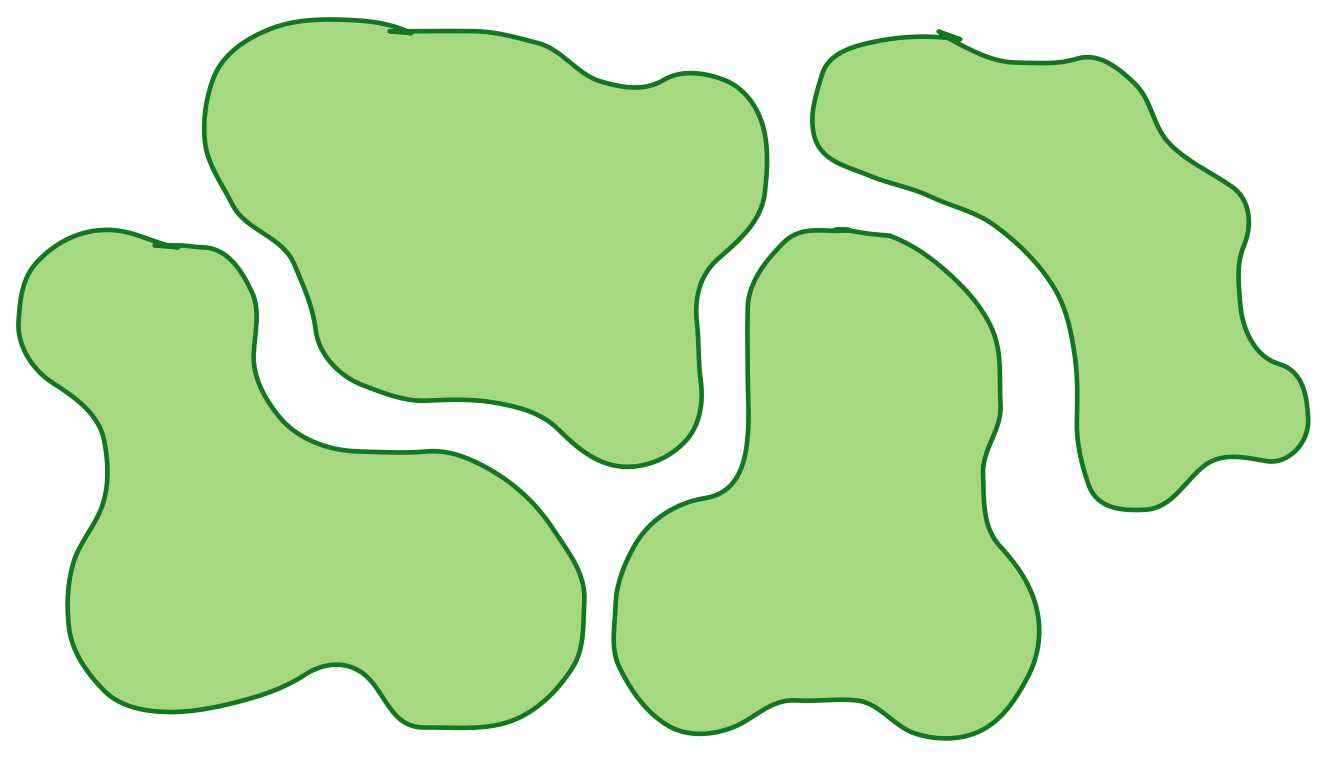
\includegraphics[width=2cm]{images/intro/objective_geom.png}};
						\node[title,font=\Large] at (1.6,0.1) {+};
						\node at (3.5,0.8) {Several Forces};
						\node[draw=none, inner sep=0pt] at (3.5,0) {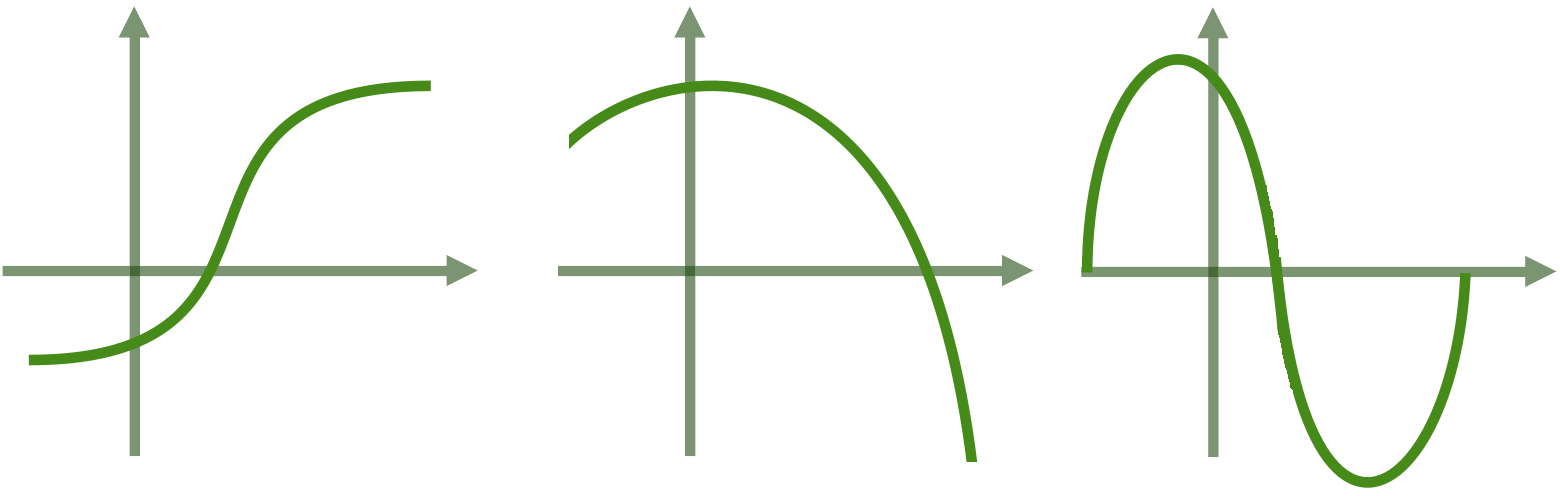
\includegraphics[width=3cm]{images/intro/objective_fct.png}};
						
						% Ajouter une flèche entre les deux rectangles
						\draw[->, title, line width=1.5pt] (5.5,0.1) -- (6.5,0.1);
						%		
						\node at (8,0.8) {Train a PINNs};
						\node[draw=none, inner sep=0pt] at (8,-0.1) {\includegraphics[width=1.5cm]{images/intro/objective_pinns.jpg}};				
					\end{tikzpicture}
				}%
			\end{figure}
			
			\textbf{ONLINE :}
			
			\vspace{-30pt}
			
			\begin{figure}[htb]
				\centering
				\resizebox{\textwidth}{!}{%
					\begin{tikzpicture}
						\node at (0,0.8) {1 Geometry - 1 Force};
						\node[draw=none, inner sep=0pt] at (0,0) {\includegraphics[width=2cm]{images/intro/objective_onegeom_onefct.png}};
						%		\node[title,font=\Large] at (1.6,0.1) {+};
						%		\node at (3.5,0.8) {Several Functions};
						%		\node[draw=none, inner sep=0pt] at (3.5,0) {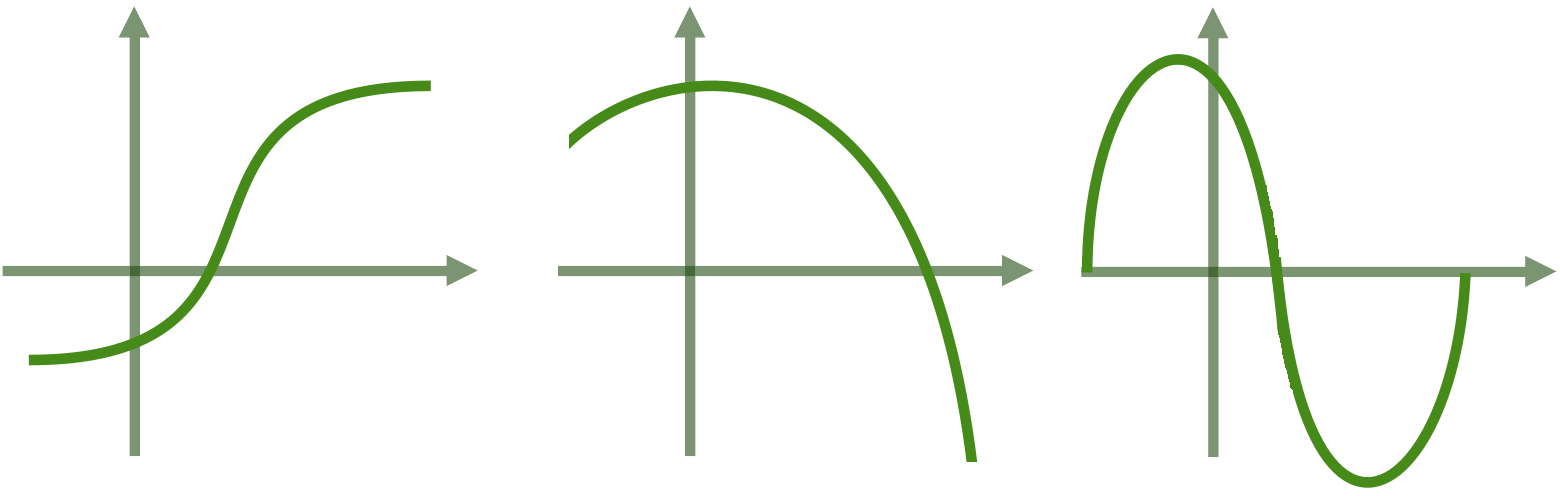
\includegraphics[width=3cm]{images/intro/objective_fct.png}};
						
						\draw[->, title, line width=1.5pt] (2,0.1) -- (3,0.1);
						
						\node[align=center] at (4,1) {Get PINNs \\ prediction};
						\node[draw=none, inner sep=0pt] at (4,-0.1) {\includegraphics[width=1.5cm]{images/intro/objective_pinns.jpg}};
						
						% Ajouter une flèche entre les deux rectangles
						\draw[->, title, line width=1.5pt] (5.5,0.1) -- (6.4,0.1);
						\draw[draw=black] (6.5,-1) rectangle ++(3,2.5);	
						\node[align=center] at (8,1) {Correct prediction \\ with $\phi$-FEM};
						\node[draw=none, inner sep=0pt] at (8,-0.1) {\includegraphics[width=2.5cm]{images/intro/objective_corr.png}};		
					\end{tikzpicture}
				}%
			\end{figure}
		\end{tcolorbox}
	\end{center}
	
	\textbf{On going work :}
	
	\small
	% \setstretch{0.5}
	\begin{itemize}
		\item Geometry : 2D, simple, fixed (as circle, ellipse..) $ \; \rightarrow \;$ 3D / complex / variable
		\item PDE : simple, static (Poisson problem) $\; \rightarrow \;$ complex / dynamic (elasticity, hyper-elasticity)
		\item Neural Network : simple and defined everywhere (PINNs) $\; \rightarrow \;$ Neural Operator
	\end{itemize}
\end{frame}

\begin{frame}{\appendixname~\theappendixframenumber~: Correction}
	\vspace{-20pt}
	\begin{figure}[htb]
		\centering
		\resizebox{\textwidth}{!}{%
			\begin{tikzpicture}
				\node at (0,0.8) {1 Geometry - 1 Force};
				\node[draw=none, inner sep=0pt] at (0,0) {\includegraphics[width=2cm]{images/hybrid/objective_onegeom_onefct.png}};
				\node at (0,-1) {$\begin{aligned}[t]
						\; \phi \quad \text{\small and} \quad &f \\
						\; (\text{\small and} \quad &g)
					\end{aligned}$};
				
				\draw[->, title, line width=1.5pt] (2,0.1) -- (3,0.1);
				
				\node[align=center] at (4,1) {Get PINNs \\ prediction};
				\node[draw=none, inner sep=0pt] at (4,-0.1) {\includegraphics[width=1.5cm]{images/hybrid/objective_pinns.jpg}};
				\node at (4,-1) {$u_{NN}=\phi w_{NN}+g$};
				
				% Ajouter une flèche entre les deux rectangles
				\draw[->, title, line width=1.5pt] (5,0.1) -- (6,0.1);
				
				\node[align=center] at (7.8,1) {Correct prediction \\ with $\phi$-FEM};
				\node[draw=none, inner sep=0pt] at (7.8,-0.1) {\includegraphics[width=2.5cm]{images/hybrid/objective_corr.png}};		
				\node at (7.8,-1) {$u_{NN}\rightarrow\tilde{u}=u_{NN}+\phi C$};
			\end{tikzpicture} 
		}%
	\end{figure}
	
	\vspace{-10pt}
	
	\textbf{Correct by adding :} Considering $u_{NN}$ as the prediction of our PINNs (trained to learn the solution of the elliptic problem), the correction problem consists in writing the solution as
	\begin{equation*}
		\tilde{u}=u_{NN}+\underset{\textcolor{blue}{\ll 1}}{\fcolorbox{blue}{white}{$\tilde{C}$}}
	\end{equation*}
	
	\vspace{-8pt}
	\begin{minipage}{\linewidth}
		\setstretch{0.5}
		and searching $\tilde{C}: \Omega \rightarrow \mathbb{R}^d$ such that
		\begin{equation*}
			\left\{\begin{aligned}
				L(\tilde{C})&=\tilde{f}, \; &&\text{in } \Omega, \\
				\tilde{C}&=0, \; &&\text{on } \Gamma,
			\end{aligned}\right. %\tag{$\mathcal{C}_{+}$} %\label{corr_add}
		\end{equation*}
		with $\tilde{f}=f-L(u_{NN})$ and $\tilde{C}=\phi C$ for the $\phi$-FEM method.
	\end{minipage}
\end{frame}
\addtocounter{appendixframenumber}{1}

\subsection{\appendixname~\theappendixframenumber~: $\phi$-FEM Method}\labelappendixframe{frame:phifem}

\begin{frame}{\appendixname~\theappendixframenumber~: Problem}
	Let $u=\phi w+g$ such that
	$$\left\{\begin{aligned}
		-\Delta u &= f, \; \text{in } \Omega, \\
		u&=g, \; \text{on } \Gamma, \\
	\end{aligned}\right.$$
	where $\phi$ is the level-set function and $\Omega$ and $\Gamma$ are given by :
	\begin{center}
		\pgfimage[width=0.5\linewidth]{images/more/PhiFEM_level_set.png}
	\end{center}
	The level-set function $\phi$ is supposed to be known on $\mathbb{R}^d$ and sufficiently smooth. \\
	For instance, the signed distance to $\Gamma$ is a good candidate.
	
	\vspace{5pt}
	
	\footnotesize
	\textit{Remark :} Thanks to $\phi$ and $g$, the boundary conditions are respected.
\end{frame}

\begin{frame}{\appendixname~\theappendixframenumber~: Fictitious domain}
	\setstretch{0.5}
	
	\vspace{10pt}
	
	\begin{center}
		\begin{minipage}{0.43\linewidth}
			\centering
			\pgfimage[width=\linewidth]{images/more/PhiFEM_domain.png}
		\end{minipage} \hfill
		\begin{minipage}{0.1\linewidth}
			\centering
			\pgfimage[width=\linewidth]{images/more/PhiFEM_fleche.png} 
		\end{minipage} \hfill
		\begin{minipage}{0.43\linewidth}
			\centering
			\pgfimage[width=\linewidth]{images/more/PhiFEM_domain_considered.png}
		\end{minipage}
	\end{center}
	
	\begin{enumerate}[\ding{217}]
		\item $\phi_h$ : approximation of $\phi$ \\ 
		\item $\Gamma_h=\{\phi_h=0\}$ : approximate boundary of $\Gamma$
		\item $\Omega_h$ : computational mesh
		\item $\partial\Omega_h$ : boundary of $\Omega_h$ ($\partial\Omega_h \ne \Gamma_h$)
	\end{enumerate}	
	
	\footnotesize
	\; \\
	\textit{Remark :} $n_{vert}$ will denote the number of vertices in each direction
\end{frame}

\begin{frame}{\appendixname~\theappendixframenumber~: Facets and Cells sets}
	
	\vspace{15pt}
	
	\begin{center}
		\begin{minipage}{0.48\linewidth}
			\centering
			\pgfimage[width=\linewidth]{images/more/PhiFEM_boundary_cells.png}
		\end{minipage} \hfill
		\begin{minipage}{0.48\linewidth}
			\centering
			\pgfimage[width=\linewidth]{images/more/PhiFEM_boundary_edges.png}
		\end{minipage}
	\end{center}
	
	\begin{enumerate}[\ding{217}]
		\item $\mathcal{T}_h^\Gamma$ : mesh elements cut by $\Gamma_h$
		\item $\mathcal{F}_h^\Gamma$ : collects the interior facets of $\mathcal{T}_h^\Gamma$ \\
		(either cut by $\Gamma_h$ or belonging to a cut mesh element)
	\end{enumerate}
	
	% \begin{minipage}{0.6\linewidth}
		%     \begin{enumerate}[\ding{217}]
			%         \item $\mathcal{T}_h^\Gamma\subset \mathcal{T}_h$ : contains the mesh elements cut by $\Gamma_h$, i.e. 
			%         \begin{equation*}
				%             \mathcal{T}_h^\Gamma=\left\{T\in\mathcal{T}_h:T\cap\Gamma_h\ne\emptyset\right\},
				%         \end{equation*}
			%         \item $\Omega_h^\Gamma$ : domain covered by the $\mathcal{T}_h^\Gamma$ mesh, i.e.
			%         \begin{equation*}
				%             \Omega_h^\Gamma=\left(\cup_{T\in\mathcal{T}_h^\Gamma}T\right)^O
				%         \end{equation*}
			%         \item $\mathcal{F}_h^\Gamma$ : collects the interior facets of $\mathcal{T}_h$ either cut by $\Gamma_h$ or belonging to a cut mesh element, i.e.
			%         \begin{align*}
				%             \mathcal{F}_h^\Gamma=\left\{E\;(\text{an internal facet of } \mathcal{T}_h) \text{ such that }\right. \\
				%             \left. \exists T\in \mathcal{T}_h:T\cap\Gamma_h\ne\emptyset \text{ and } E\in\partial T\right\}
				%         \end{align*}
			%     \end{enumerate}
		% \end{minipage}
\end{frame}

\begin{frame}{\appendixname~\theappendixframenumber~: Poisson problem}
	\textbf{Approach Problem :} Find $w_h\in V_h^{(k)}$ such that 
	$$a_h(w_h,v_h) = l_h(v_h) \quad \forall v_h \in V_h^{(k)}$$
	where
	$$a_h(w,v)=\int_{\Omega_h} \nabla (\phi_h w) \cdot \nabla (\phi_h v) - \int_{\partial\Omega_h} \frac{\partial}{\partial n}(\phi_h w)\phi_h v+\fcolorbox{blue}{white}{$G_h(w,v)$},$$
	$$l_h(v)=\int_{\Omega_h} f \phi_h v + \fcolorbox{blue}{white}{$G_h^{rhs}(v)$} \qquad \qquad \color{blue}\text{Stabilization terms}$$
	and 
	$$V_h^{(k)}=\left\{v_h\in H^1(\Omega_h):v_{h|_T}\in\mathbb{P}_k(T), \; \forall T\in\mathcal{T}_h\right\}.$$
	For the non homogeneous case, we replace
	$$u=\phi w \quad \rightarrow \quad u=\phi w+g$$ 
	by supposing that $g$ is currently given over the entire $\Omega_h$.
\end{frame}

\begin{frame}{\appendixname~\theappendixframenumber~: Stabilization terms}
	\begin{center}
		\centering
		\pgfimage[width=\linewidth]{images/more/PhiFEM_stab_terms.png}
	\end{center}
	\small
	\underline{1st term :} ensure continuity of the solution by penalizing gradient jumps. \\
	$\rightarrow$ Ghost penalty [Burman, 2010] \\
	\underline{2nd term :} require the solution to verify the strong form on $\Omega_h^\Gamma$. \\
	\normalsize
	\textbf{Purpose :} 
	\begin{enumerate}[\ding{217}]
		\item reduce the errors created by the "fictitious" boundary 
		\item ensure the correct condition number of the finite element matrix
		\item restore the coercivity of the bilinear scheme
	\end{enumerate}
\end{frame}
\addtocounter{appendixframenumber}{1}

\subsection{\appendixname~\theappendixframenumber~: Results}\labelappendixframe{frame:results}

\begin{frame}{\appendixname~\theappendixframenumber~: Problem considered}
	\textbf{PDE :} Poisson problem with Homogeneous Dirichlet conditions \\
	Find $u : \Omega \rightarrow \mathbb{R}^d (d=1,2,3)$ such that
	\begin{equation*}
		\left\{
		\begin{aligned}
			-\Delta u &= f, \; &&\text{in } \; \Omega, \\
			u&=0, \; &&\text{on } \; \Gamma,
		\end{aligned}
		\right.
	\end{equation*}
	with $\Delta$ the Laplace operator, $\Omega$ a smooth bounded open set and $\Gamma$ its boundary. \\
	
	\textbf{Geometry :} Circle - center=$(0.5,0.5)$ , radius=$\sqrt{2}/4$ \\
	\begin{minipage}{0.3\linewidth}
		\centering
		\pgfimage[width=0.9\linewidth]{images/more/circle.png}
	\end{minipage} \;
	\begin{minipage}{0.68\linewidth}
		\begin{enumerate}[\ding{217}]
			\item \textbf{Level-set function : }
			$$\phi(x,y)=-1/8+(x-1/2)^2+(y-1/2)^2$$
			
			\item \textbf{Exact solution :} 
			
			\begin{equation*}
				u_{ex}(x,y) = \phi(x,y)\sin(x)\exp(y)
			\end{equation*} 
		\end{enumerate}
	\end{minipage}
\end{frame}

\begin{frame}{\appendixname~\theappendixframenumber~: Networks}
	\textbf{PINNs :} Multi-Layer Perceptron (MLP, Fully connected) with a physical loss

	\begin{minipage}{0.58\linewidth}
		\centering
		\pgfimage[width=0.6\linewidth]{images/more/MLP_schema.png}
		
		\setstretch{0.2}\small
		\begin{itemize}[\ding{217}]
			\item n\_layers=4
			\item n\_neurons=20 (in each layer)
			\item n\_epochs=10000
			\item n\_pts=2000 (randomly drawn in the square $[0,1]^2$)
		\end{itemize}
	\end{minipage} \quad
	\begin{minipage}{0.38\linewidth}
		\begin{center}
			$loss = mse(\Delta (\phi(x_i,y_i)w_{\theta,i})+f_i)$
			
			\vspace{1.5pt}
			
			\pgfimage[width=0.5\linewidth]{images/more/PINNs_explanation.png}
		\end{center}
		
		with $(x_i,y_i)\in\mathcal{O}$.
		
		\small
		\textit{Remark :} We impose exact boundary conditions.
	\end{minipage}

	\vspace{5pt}

	\textbf{Some important points :}
	\begin{itemize}[\textbullet]
		\item Need $u_{NN}\in\mathbb{P}^k$ of high degree (PINNs Ok)
		\item Need the derivatives to be well learn (PINNs Ok)
		\item For the correction : Need a correct solution on $\Omega_h$, not on $\Omega$ (training on the square for the moment).
	\end{itemize}
\end{frame}

\begin{frame}{\appendixname~\theappendixframenumber~: Training}
	\begin{center}
		\pgfimage[width=\linewidth]{images/more/solution_config0.png}
	\end{center}
	
	{\fontencoding{U}\fontfamily{futs}\selectfont\char 49\relax} We consider a single problem ($f$ fixed) on a single geometry ($\phi$ fixed).
	 
	$$||u_{ex}-u_\theta||_{L^2(\Omega)}^{(rel)}\approx 2.81e-3$$
\end{frame}

\begin{frame}{\appendixname~\theappendixframenumber~: Correction}
	$u_\theta\in\mathbb{P}^{10} \; \rightarrow \; \tilde{u}\in\mathbb{P}^1$
	
	\begin{minipage}{0.5\linewidth}
		\centering
		\pgfimage[width=\linewidth]{images/more/time_precision.png}
		
		\raggedright
		FEM / $\phi$-FEM : $n_{vert}\in\{8,16,32,64,128\}$
		
		Corr : $n_{vert}\in\{5,10,15,20,25,30\}$
	\end{minipage} \quad
	\begin{minipage}{0.46\linewidth}
		\centering
		\pgfimage[width=\linewidth]{images/more/results_time_1e-4.png}
		
		\tiny\raggedright
		\textit{Remark :} Problem with assemble and solve time \\
		+ mesh time for $\phi$-FEM would be parallelized
		
		\small
		$\textbullet$ \textbf{mesh} - FEM : construct the mesh \\
		($\phi$-FEM : construct cell/facet sets) \\
		$\textbullet$ \textbf{u\_PINNs} - get $u_\theta$ in $\mathbb{P}^{10}$ freedom degrees \\
		$\textbullet$ \textbf{assemble} - assemble the FE matrix \\
		$\textbullet$ \textbf{solve} - resolve the linear system
	\end{minipage}
	
	\small
	\textit{Remark :} The stabilisation parameter $\sigma$ of the $\phi$-FEM method has a major impact on the error obtained.
\end{frame}
\addtocounter{appendixframenumber}{1}


